As said in the conclusion of the previous sub-chapter, Stratum protocol was born during the same period of getblocktemplate, in the second half of 2012.
The main developer and proposer of Stratum was Marek Palatinus (aka "slush"), who was the founder of one of the first Bitcoin mining pools, called \textit{slushpool}. He announced this new protocol on \textbf{11th September 2012}, in a thread on Bitcoin Talk Forum \cite{bitcointalkANNStratum}.

\begin{figure}[h!]
    \centering
    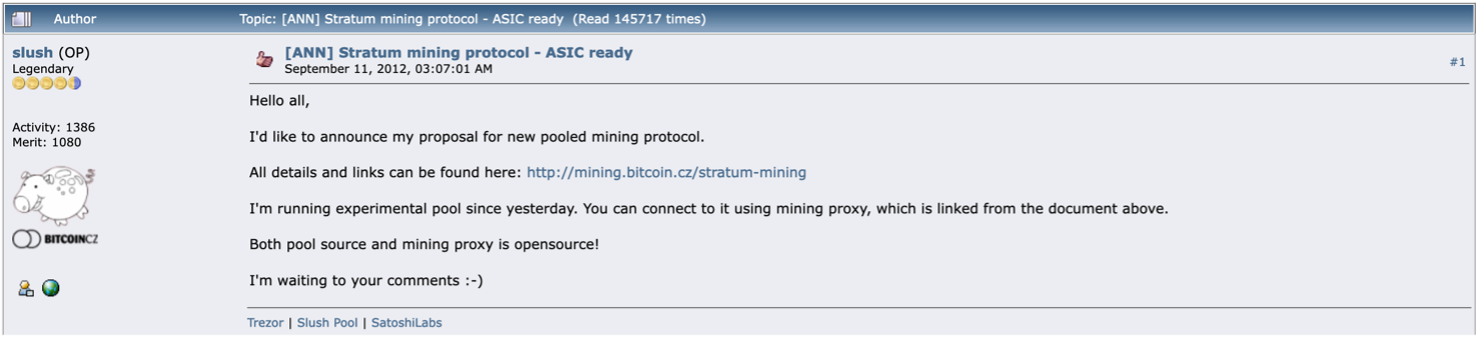
\includegraphics[width=15cm]{Figures/stratum/stratum1.png}
    \caption{Slush \textit{stratum}  announcement, Bitcoin Talk Forum}
    \label{fig:stratum1}
\end{figure}

\noindent The reason which took \textit{slush} to develop Stratum, was the same as \textit{getblocktemplate}'s: the mining protocol used at that time (\textit{getwork}) was not efficient anymore, due to the newest more powerful mining equipment, which was coming, in addition to the ever-growing pooled mining activities. 
As discussed in the announcement thread, \textit{getwork} permitted just 32 bits manipulation for the nonce research (in most cases they could also change the timestamp field, thanks to the nTime-rolling extension supported by most of the pools), so frequent requests from miners to mining pool server were needed to get new jobs to work on.\\ 
The other bad aspect of \textit{getwork} was related to the necessity of HTTP protocol to transport the JSON-RPC methods: since HTTP is a protocol which is most suitable for websites navigation, it was not ideal for Bitcoin mining operations. With the growing global hashrate of that time, it was revealing very inefficient to manage the frequent requests coming from miners, especially for what regards the load on the pool servers and the bandwidth needed.
As we have seen in \ref{sec:longpolling}, a mitigation that was implemented in the \textit{getwork} protocol was the exploitation of Long Polling extension. However, its usage led to another issue: the packet storms which were received by the pool server from the miners who were trying to reconnect to the server after long polling broadcasts: most of the times it was hard to distinguish long polling re-connections from possible DDoS attacks.\\
For these reasons, \textit{getwork} was totally unable to scale pooled mining operations: that's why Stratum was designed very differently from it.\\\\
To investigate more deeply upon the architectural choices of Stratum protocol, it can be useful to look at the draft protocol specifications present in a publicly shared Google document \cite{googleStratumNetwork}.
